\chapter{Introduction}
% \setstretch{1.5}

\section{Introduction}

    \lipsum[1]

    \begin{figure}[ht]
        \centering
        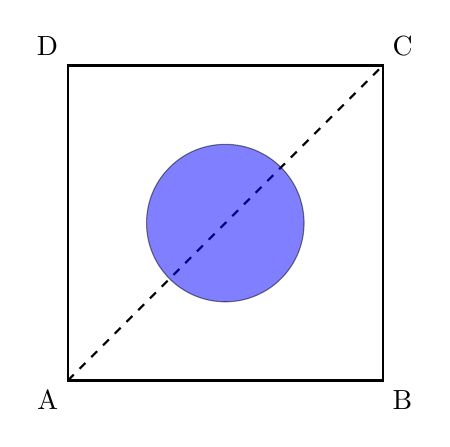
\begin{tikzpicture}
            % Define some coordinates
            \coordinate (A) at (0,0);
            \coordinate (B) at (4,0);
            \coordinate (C) at (4,4);
            \coordinate (D) at (0,4);
    
            % Draw a rectangle
            \draw[thick] (A) -- (B) -- (C) -- (D) -- cycle;
    
            % Label the corners
            \node[below left] at (A) {A};
            \node[below right] at (B) {B};
            \node[above right] at (C) {C};
            \node[above left] at (D) {D};
    
            % Draw a diagonal line
            \draw[thick, dashed] (A) -- (C);
    
            % Draw a circle at the center
            \draw[fill=blue, opacity=0.5] (2,2) circle (1cm);
        \end{tikzpicture}
        \caption{Sample TikZ Figure: A rectangle with a diagonal and a circle at the center.}
        \label{fig:sample}
    \end{figure}
    
    \lipsum[2]
    
    \lipsum[3]

\section{Problem Statement} 

    \lipsum[1]
    
    \begin{table}[ht]
        \centering
        \caption{Sample Table: Comparison of Items Across Categories}
        \begin{tabular}{lccc}
            \toprule
            \textbf{Category} & \textbf{Item 1} & \textbf{Item 2} & \textbf{Item 3} \\
            \midrule
            Category A & 10 & 20 & 30 \\
            Category B & 15 & 25 & 35 \\
            Category C & 20 & 30 & 40 \\
            \bottomrule
        \end{tabular}
        \label{tab:sample}
    \end{table}

\section{Objectives} 

    \lipsum[1]

\section{Scope and Limitation} 

    \lipsum[1]


\section{Report Organization} 

    \lipsum[1]

    \begin{figure}[ht]
        \centering
        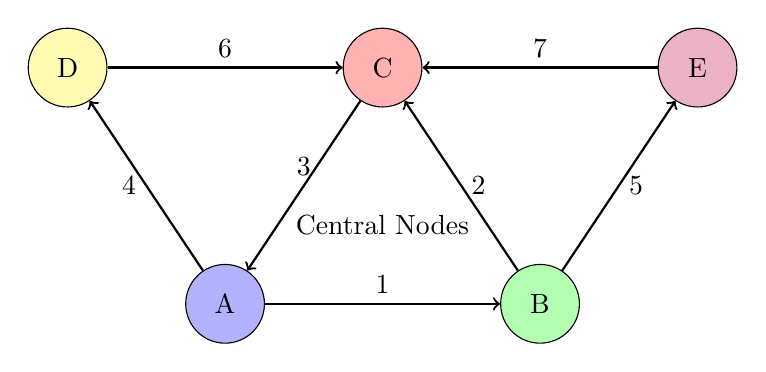
\begin{tikzpicture}
            % Define nodes
            \node[draw, circle, fill=blue!30, minimum size=1cm] (A) at (0,0) {A};
            \node[draw, circle, fill=green!30, minimum size=1cm] (B) at (4,0) {B};
            \node[draw, circle, fill=red!30, minimum size=1cm] (C) at (2,3) {C};
            \node[draw, circle, fill=yellow!30, minimum size=1cm] (D) at (-2,3) {D};
            \node[draw, circle, fill=purple!30, minimum size=1cm] (E) at (6,3) {E};
            
            % Draw edges
            \draw[->, thick] (A) -- (B) node[midway, above] {1};
            \draw[->, thick] (B) -- (C) node[midway, right] {2};
            \draw[->, thick] (C) -- (A) node[midway, above] {3};
            \draw[->, thick] (A) -- (D) node[midway, left] {4};
            \draw[->, thick] (B) -- (E) node[midway, right] {5};
            \draw[->, thick] (D) -- (C) node[midway, above] {6};
            \draw[->, thick] (E) -- (C) node[midway, above] {7};
    
            % Add labels
            \node at (2,1) {Central Nodes};
        \end{tikzpicture}
        \caption{Sample Diagram: Nodes and Connections with Labels}
        \label{fig:network}
    \end{figure}